% !TeX root = RJwrapper.tex
\title{Conference Report of Why R? Turkey 2021}
\author{by Mustafa Cavus, Olgun Aydin, Ozan Evkaya, Ozancan Ozdemir, Deniz Bezer, Ugur Dar}

\maketitle

\abstract{
The Why R? Turkey 2021 as a three-day online conference was organized to bring together researchers and professionals from Turkey on April 16-17-18, 2021. We hereby aimed to promote the R community in Turkey by bringing R users with different backgrounds such as genetics, sociology, finance, economy, bio-statistics. There were 8 thematic sessions and 18 invited speakers. In this article, it is aimed to describe the preparation phase, technical details, and the impact of the conference on audience.}

\section{Why R? Turkey 2021}

The \href{whyr.pl/2021/turkey/}{Why R? Turkey 2021} is a pre-meeting of Why R? 2021 conference. Why R? conferences are international conference series organized annually by the \href{whyr.pl}{Why R? Foundation} since 2017. It is one of the largest annual R conferences in Central Europe \citep{why2019}. In addition to the main conference, pre-meetings are held in different cities from all over the world. In 2017, four pre-meetings were organized in Poland. Thereafter, eleven pre-meetings across four different countries were held in 2018. In 2019, twelve pre-meetings took place in eight different countries. In 2020, in a pre-meeting framework, totally  six organizations appeared in four different countries (Poland (2), Turkey (2), Ireland (1), and Germany (1)). Among those six pre-meetings, two of them were held in Istanbul (24.04.2020) and Ankara (27.04.2020) consecutively, as a one-day organization \citep{whyrEvents}. \\

\begin{figure}[h]
  \centering
  
\includegraphics[width=0.4\textwidth]{logo.png}
  \caption{The logo of Why R? Turkey 2021.}
  \label{figure:rlogo}
\end{figure} 

Two primary goals of Why R ? Turkey 2021 are; 

\begin{enumerate}
    \item to bring together Turkish R users from all over the world
    \item to broaden the horizon of the students with respect to the diverse disciplines
\end{enumerate}

%the first one was to bring together Turkish R users from all over the world and the second one is to broaden the horizon of the students with respect to the diverse disciplines . 

For this purpose, experienced researchers, who are R users, from various disciplines were invited to the conference as a speaker.  The conference program was designed comprehensively to cover various research fields such as bio-statistics, sociology, educational sciences, psychology, molecular biology, genomics, football analytics, and economics. The detailed program is shown in Table \ref{tab:prog}. 

\section{Participants}

There were 2180 registered participants, 60\% were students and 40\% were professionals who work for governmental institutions, companies from the private sector, and academicians from the universities in Turkey. With regards to the education level of the student participants, 50\% of them was graduate and rest was undergraduate students. 60\% of the students study Statistics. The number of unique participants for the conference is 880. Additionally, the share of each thematic session is counted as 540, 435, 380, 355, 390, 360, respectively. The whole event was organized and moderated by the organization committee including 6 members.

Most of the participants were registered from İstanbul, Ankara, and İzmir, respectively. In the conference, we had participants from 73 provinces out of 81 provinces in Turkey. The distribution of registered participants by provinces is illustrated in Figure \ref{fig2}. 

\begin{figure}[!h]
    \centering
    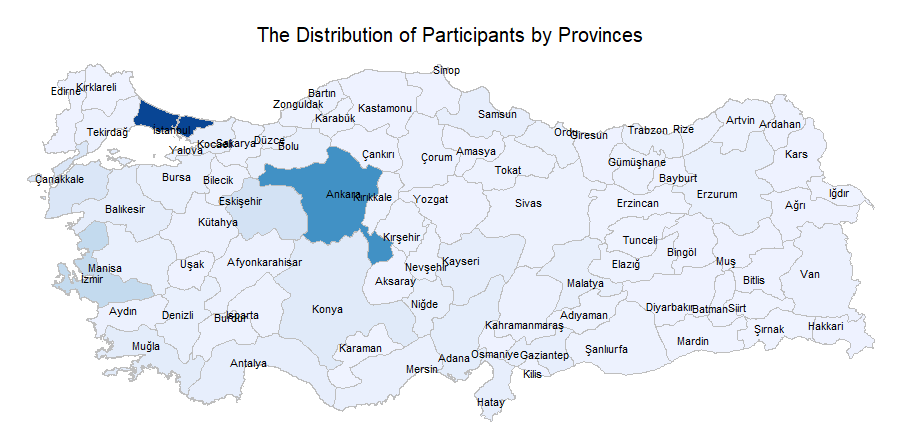
\includegraphics[width=0.75\textwidth]{whyr_map.png}
    \caption{The Distribution of Participants by Provinces}
    \label{fig2}
\end{figure}

In addition to Turkey, we had participants from the USA, England, Belgium, Sweden, Switzerland, Qatar, Nederland, Italy, France, and Spain. In that respect, the conference was successful to bring Turkish R users from different countries as well. 

\section{Conference Program}
{
The detailed conference program, shown in Table \ref{tab:prog}, consists of 6 main sessions over three days. For each speaker, there were 30 minutes to complete his/her presentation and thereafter the participants are guided to the breakout rooms in the Zoom platform for Q\&A session with the speaker.  

\begin{table}[h]
    \centering
    \begin{tabular}{p{1cm}p{4cm}p{6cm}}\hline
         \textbf{Session} &\textbf{Speaker} & \textbf{Title} \\\hline
         
         & Gökmen Zararsız & Using R in Medicine and Diagnostic Domains: The Case of the Alzheimer Project \vspace{2mm}\\\cline{2-3}
         
         1 & Dinçer Göksülük & BioSoft: A cloud-based platform for Biostatistics/Bioinformatics softwares developed using R programming language \vspace{2mm}\\\cline{2-3}
         
         & Erdal Coşgun & Genetic research on cloud-based systems: The Bioconductor experience \vspace{2mm}\\\hline
         
         & Tuba Bircan & R for whom? \vspace{2mm}\\\cline{2-3}
         
         2& Gökhan Kaya & Data Analysis and using theory in R for sociological researches: Opportunities and challenges \vspace{2mm}\\\cline{2-3}
         
         & Dilek Yıldız & Using R in demography \vspace{2mm}\\\cline{2-3}
         
         & Ali O. İlhan & R and bibliometric analysis: a brief introduction \vspace{2mm}\\\hline
         
         & Kadir Kızılkaya & Using R for animal breeding and genomic selection\vspace{2mm}\\\cline{2-3}
         
         3& Hilal Özkılınç & Using R in genomics studies \vspace{2mm}\\\cline{2-3}
         
         & Burcu Mestav & Using R in aquaculture and ecology \vspace{2mm}\\\hline
         
         & Mehmet Can Demir & Research studies in educational science using R  \vspace{2mm}\\\cline{2-3}
         
         4& Kübra Atalay Kabasakal & R packages for educational science \vspace{2mm}\\\cline{2-3}
         
         & Eren Halil Özberk & Using R in psychology\vspace{2mm}\\\hline
         
         & Yeşim Güney & Structural Breakpoints in Turkey COVID-19 data \vspace{2mm}\\\cline{2-3}
         
        5 & İpek Güler & R packages for joint modeling of survival and recurrent data\vspace{2mm}\\\cline{2-3}
         
         & Emre Toros & Soccer, data, why, how, and R\vspace{2mm}\\\hline
         
         & Burak Saltoğlu & Behavioral financial analysis by using R\vspace{2mm}\\\cline{2-3}
         
         6& Ahmet Akgül & Regression analysis in R: house price prediction model for Istanbul\vspace{2mm}\\\cline{2-3}
         
         & Ayhan Yüksel & Algoritmic trade using R\vspace{2mm}\\\hline
    \end{tabular}
    \caption{Program of the Why R? Turkey 2021}
    \label{tab:prog}
\end{table}
}

\section{Promotion of the Event and Reactions}

The social media channels (Instagram, Twitter, Facebook and, LinkedIn) were used for the promotion of the conference. Conference social media accounts were created to conduct the promotion except LinkedIn. Organization committee members' personal LinkedIn accounts were preferred to promote the event.

Instagram ads were used to reach out bigger audience. Advertisements went live two weeks before starting date of the conference and finished 4 days before the conference started. At the end of this period, we obtained more than 500 followers most of whom are young adults as shown in Figure \ref{fig3}.  Besides, the Instagram account of the conference was visited more than 2.000 times during the advertisement period.

\begin{figure}[!h]
    \centering
    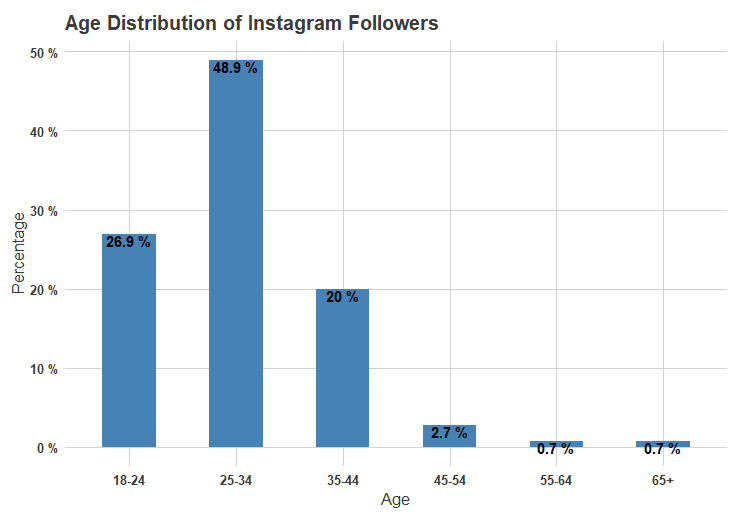
\includegraphics[width=0.75\textwidth]{insta_followers.png}
    \caption{Age Distribution of Instagram Followers}
    \label{fig3}
\end{figure}

In addition to Instagram, Twitter was also used efficiently for the promotion. The Twitter account for this event was created in January, but the posts started to be shared at the end of February. To reach R users, all contents were posted using the \texttt{\#Rstats} hashtag. As of May 8, the Twitter account of the conference was visited by more than 18000 users, and tweets were viewed more than 174000 times. 

According to our calendar, we started to share our posts once a week on Twitter. Although post frequency was lower at the beginning, the number of followers reached over three hundreds quickly. However, the account gained the highest number of followers in April. (Figure \ref{fig4}). 

\begin{figure}[h]
    \centering
    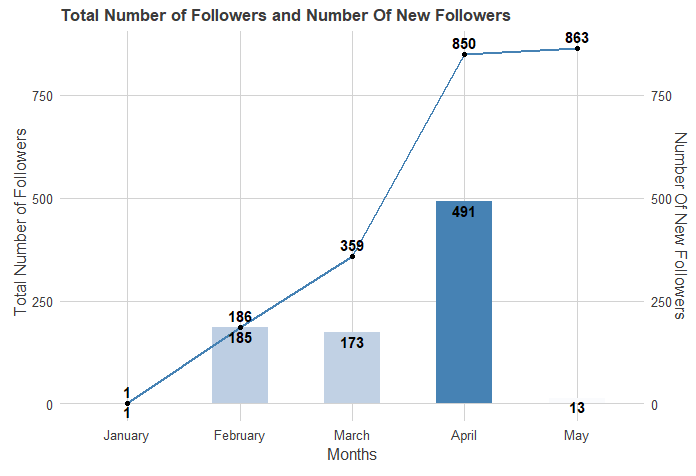
\includegraphics[width=0.75\textwidth]{whyr_twiter.png}
    \caption{Evolution of the number of followers of the WhyR? Turkey 2021 Twitter Account}
    \label{fig4}
\end{figure}

Thus, visits and view statistics of the Twitter account show that Twitter was the most efficient platform to reach R users. 


\section{Technical Solutions}

The official website was developed and used as the primary information source for the conference. The website was hosted on \href{whyr.pl}{Why R? Foundation's domain}. This allowed us to be more visible on Google Search. The abstract book was prepared using the bookdown R package and was served via the website.

Instant updates in terms of program, speakers, program, schedule, were shared with the audience via Instagram, and Twitter accounts, dedicated to the conference. Twitter and Instagram account caught the attention of people interested in participating in the conference very quickly.

Google Forms was preferred for registration purposes and used as a contact form. Hyperlinks to the registration form and contact form were added to the website. During registration, participants were asked to answer questions regarding their professional background, education level, R knowledge. Thanks to this, we had a chance to better understand participants' profiles.

All speeches were streamed on Zoom. Premium zoom account was purchased to be able to have 1000 participants online at the same time. Separate zoom meetings were set for each session. After each talk, dedicated breakout rooms were created and Q\&A sessions were conducted in breakout rooms. This allowed the audience to have more interaction with speakers. The cost of the Zoom account was covered by the funding received from Why R? Foundation and R Consortium. URLs for the recordings, as well as slide decks and R scripts used by speakers during presentations, shared publicly on the \href{https://github.com/whyr2021turkey/Konusmalar}
{GitHub repository} of the conference.

%%%%%%%%%%%%%%%%%%%%%%%%%%%%%%%%%%%%%%%%%%%%%%%%%%%%%%%%%%
%\section{Participant pattern}

%The number of unique participants for the conference is 880. Additionally, the share of each thematic session is counted as 1-540, 2-435, 3-380, 4-355, 5-390, 6-360 

%This section may contain a figure such as Figure~\ref{figure:rlogo}.

%\textcolor{red}{OE: Burada da basit bir barplot iyi olur, genel ile uyum açısından. Sadece sayılar yerine}

%\textcolor{blue}{MC: Bu kısmı tamamen bir yere eklerim diye, not etmek için yazmıştım. Buradaki bilgileri \textbf{Participants} bölümüne ekliyorum. Bu bölümü uçurabiliriz.}

%\textcolor{brown}{OA: Bence de direkt ucuralim.}
%%%%%%%%%%%%%%%%%%%%%%%%%%%%%%%%%%%%%%%%%%%%%%%%%%%%%%%%%%
\newpage
\section{Summary}

The three-day online conference of Why R? Turkey 2021 aimed to bring R users from different fields and make a connection between the Turkish R users and possible future users from various disciplines. In that respect, the attained total number of participants, the fruitful Q\&A sessions and the overall positive attitudes from all speakers/participants revealed that the meeting reached its main objective. To sum up, Why R? Turkey 2021 is the best comprehensive online meeting held for Turkish R users and it promises both national and international organizations in the near future. 

%%%%%%%%%%%%%%%%%%%%%%%%%%%%%%%%%%%%%%%%%%%%%%%%%%%%%%%%%%
\section{Acknowledgment}
We would like to thank all the sponsors that support the organization of Why R? Turkey 2021: \href{http://whyr.pl/foundation/about/}{Why R? Foundation}, \href{https://www.r-consortium.org}{R Consortium}, and \href{https://www.stickermule.com}{StickerMule}. 

%%%%%%%%%%%%%%%%%%%%%%%%%%%%%%%%%%%%%%%%%%%%%%%%%%%%%%%%%%
\section{Additional Information}
Further information about Why R? Turkey 2021 and the contributions presented during the conference can be found at the following links:

\begin{itemize}
    \item Website: \url{http://whyr.pl/2021/turkey/}
    \item Twitter: \url{https://twitter.com/whyr2021turkey} 
    \item YouTube Channel: \url{https://www.youtube.com/channel/UCr8qT7gK9WQZjCNz7Agi7sA}
    \item Materials: \url{https://github.com/whyr2021turkey}
    \item Abstract Book: \url{http://whyr.pl/2021/turkey/abstract_book/}
\end{itemize}


%%%%%%%%%%%%%%%%%%%%%%%%%%%%%%%%%%%%%%%%%%%%%%%%%%%%%%%%%%
\bibliography{RJreferences}

%%%%%%%%%%%%%%%%%%%%%%%%%%%%%%%%%%%%%%%%%%%%%%%%%%%%%%%%%%
\newpage
\address{Mustafa Cavus\\
  Eskisehir Technical University\\
  Department of Statistics\\
  Eskisehir, Turkey\\
  \url{https://orcid.org/0000-0002-6172-5449}\\
  \email{mustafacavus@eskisehir.edu.tr}}

\address{Olgun Aydın\\
  Gdańsk University of Technology\\
  Gdańsk, Poland\\
  Department of Statistics\\
  \url{https://orcid.org/0000-0002-7090-0931}\\
  \email{olgun.aydin@pg.edu.pl}}

\address{Ozan Evkaya\\
  Padova University\\
  Department of Statistical Sciences\\
  Padova, Italy\\
  \url{https://orcid.org/0000-0002-5076-8144}\\
  \email{ozanevkaya@gmail.com}}
  
\address{Ozancan Ozdemir\\
  Middle East Technical University\\
  Department of Statistics\\
  Ankara, Turkey\\
  \url{https://orcid.org/0000-0002-7850-3885}\\
  \email{ozancan@metu.edu.tr}}
  
\address{Deniz Bezer\\
  Middle East Technical University\\
  Department of Statistics\\
  Ankara, Turkey\\
  \email{deniz.bezer@metu.edu.tr}}
  
\address{Ugur Dar\\
  Eskisehir Technical University\\
  Department of Statistics\\
  Eskisehir, Turkey\\
  \email{ugurdar@eskisehir.edu.tr}}

